\documentclass[12pt]{ctexart}
\usepackage{amsmath,amssymb,graphicx,geometry}
\geometry{a4paper, margin=1in}
\graphicspath{{./images/}}
\usepackage{caption}
\usepackage{hyperref}
\title{低空复杂环境下的多无人机协同路径覆盖与任务分配研究}
\author{金泊宇\and 田佳豪 \and 曹阳}
\date{\today}

\begin{document}

\maketitle

\begin{abstract}
在灾害救援、军事侦察、应急物资投送等任务中,多无人机协同执行覆盖任务具有重要意义。本文围绕在低空复杂环境中,多无人机协同路径规划与任务分配的问题,建立数学模型并提出相应的分配与路径优化算法,结合贪心策略与协同控制机制,实现任务完成、避障、安全返航与充电策略的统一优化。最后,通过实例模拟验证模型有效性。
\end{abstract}

\section{引言}
随着无人机技术的快速发展,群体协同飞行被广泛应用于覆盖式侦察、物资投放等任务。在低空复杂环境中,存在动态障碍、通信限制与能源约束,增加了路径规划与任务调度的复杂度。本文重点研究如下问题:
\begin{itemize}
    \item 路径优化:如何在最短总飞行距离或时间下完成目标点覆盖;
    \item 通信与安全:无人机间需保持通信与降落安全间距;
    \item 动态变化:任务过程中出现新的目标点或障碍;
    \item 能源管理:需考虑统一返航与充电机制。
\end{itemize}

\section{问题描述与建模}

\subsection{任务基本约束}
\begin{itemize}
    \item 无人机最大飞行速度为 50 m/s,可瞬时转向。
    \item 最长续航时间不超过 600 s,需预留返航时间。
    \item 无人机间距不低于 50 m,通信范围不超过 1 km。
    \item 降落时无人机之间保持最小安全间隔(时间/空间)。
    \item 每个目标点需被至少一架无人机访问一次。
\end{itemize}

\subsection{模型变量定义}
设有 $m$ 架无人机 $U_1, \dots, U_m$,$n$ 个目标点 $T_1, \dots, T_n$,目标点坐标为 $(x_i, y_i)$。

\begin{itemize}
    \item $d_{ij}$:无人机 $U_i$ 到目标点 $T_j$ 的距离;
    \item $C_i$:无人机 $U_i$ 的剩余续航时间;
    \item $a_{ij}$:若 $U_i$ 执行 $T_j$,则 $a_{ij} = 1$,否则为 0;
    \item $L$:任务总耗时或飞行总距离。
\end{itemize}

\section{算法设计}

\subsection{长机-僚机协同机制}
指定一架长机,采用贪心策略优先访问高优先级目标点,其他僚机在保持通信约束内,自主完成周边任务,并向长机靠拢。

\subsection{任务分配与返航机制}
每次任务分配时,考虑如下因素:
\begin{itemize}
    \item 当前无人机是否具备完成任务的载重或悬停能力;
    \item 执行任务 + 返回起点是否在剩余续航时间内;
    \item 一旦任一无人机续航不足,全队集体返航并充电;
    \item 返回时降落延迟分布,保证最小间距。
\end{itemize}

\subsection{避障策略}
若某路径穿过障碍区域,则采用最短绕行策略(可拓展为 A*、RRT 等);同时若僚机绕障碍导致脱离编队,全队等待其归位后继续。

\section{模拟实验与结果}
以如下无人机参数与任务集为例:

\begin{center}
\begin{tabular}{|c|c|c|c|}
\hline
无人机 & 最大载重 (kg) & 最大续航时间 (s) & 侦察悬停时间 (s) \\
\hline
U1 & 15 & 500 & 30 \\
U2 & 10 & 600 & 60 \\
U3 & 20 & 450 & 20 \\
\hline
\end{tabular}
\end{center}

任务示例包含 10 个目标点,涵盖紧急/普通物资投放与侦察任务,优先级从高到低排序。具体路径与任务完成情况如下图所示。

\begin{figure}[h]
    \centering
    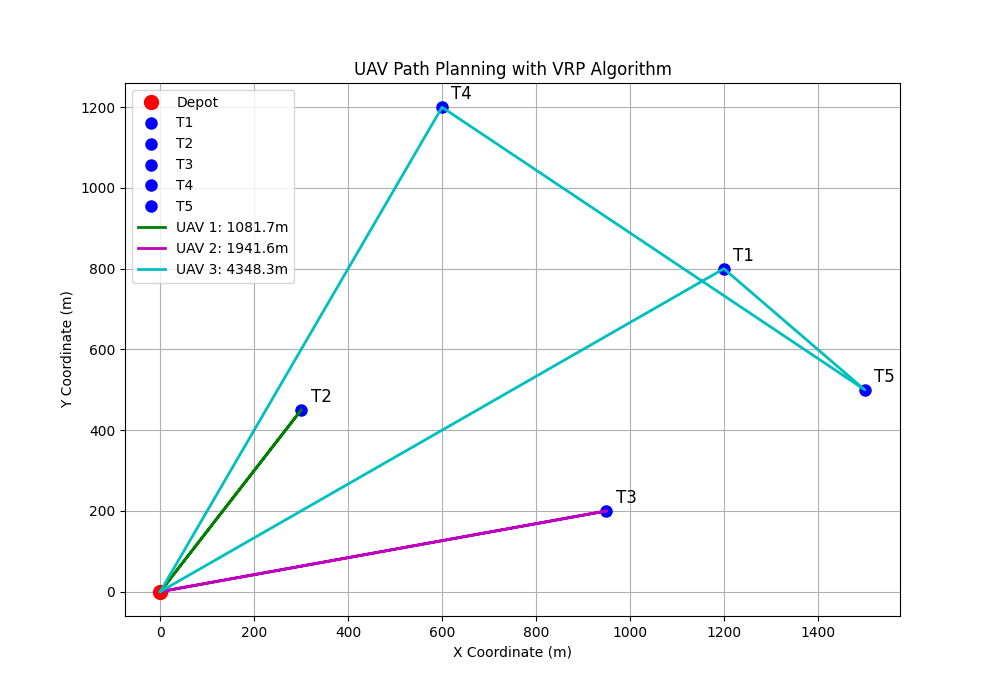
\includegraphics[width=0.8\textwidth]{example-path.png}
    \caption{无人机任务路径示意图}
\end{figure}

\section{结论}
本文建立了适用于低空复杂环境的多无人机路径与任务协同模型,引入长机-僚机机制与能源管理策略。通过统一返航、避障规避、任务优先级排序等手段,实现了协同高效执行多目标任务的路径优化,为实际部署提供理论参考。

\end{document}
